\documentclass[10pt,tikz,border=5pt]{standalone}
\usepackage{lmodern}
\usetikzlibrary{shapes.geometric}
\begin{document}
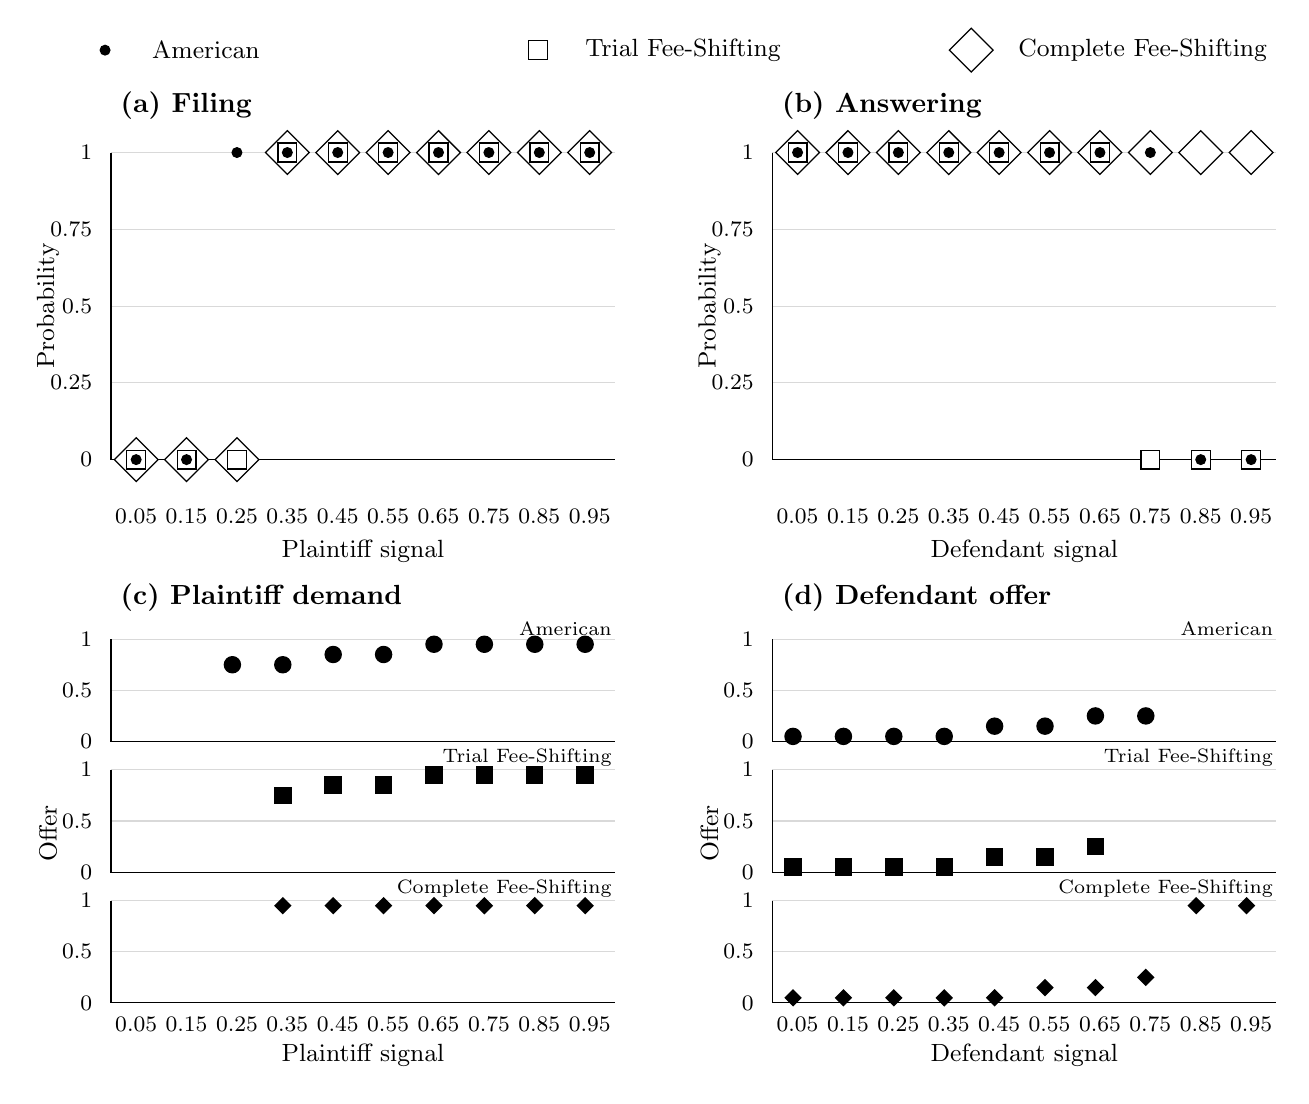
\begin{tikzpicture}[font=\small]\node[draw=black,fill=black,circle,inner sep=0pt,minimum size=3.5pt,line width=.45pt] at (0.925,12.95) {};
\node[anchor=west] at (1.4,12.95) {American};
\node[draw=black,fill=white,rectangle,inner sep=0pt,minimum size=6.8pt,line width=.45pt] at (6.425,12.95) {};
\node[anchor=west] at (6.9,12.95) {Trial Fee-Shifting};
\node[draw=black,fill=white,diamond,aspect=1,inner sep=0pt,minimum size=16pt,line width=.45pt] at (11.925,12.95) {};
\node[anchor=west] at (12.4,12.95) {Complete Fee-Shifting};
\node[anchor=west,font=\bfseries] at (1,12.25) {(a) Filing};
\begin{scope}[shift={(1,7.75)},x=6.4cm,y=3.9cm]
\draw[black!15] (0,0)--(1,0);
\node[anchor=east,font=\footnotesize] at (-.018,0) {0};
\draw[black!15] (0,0.25)--(1,0.25);
\node[anchor=east,font=\footnotesize] at (-.018,0.25) {0.25};
\draw[black!15] (0,0.5)--(1,0.5);
\node[anchor=east,font=\footnotesize] at (-.018,0.5) {0.5};
\draw[black!15] (0,0.75)--(1,0.75);
\node[anchor=east,font=\footnotesize] at (-.018,0.75) {0.75};
\draw[black!15] (0,1)--(1,1);
\node[anchor=east,font=\footnotesize] at (-.018,1) {1};
\draw (0,1)--(0,0)--(1,0);
\node[anchor=north,font=\footnotesize] at (0.05,-.13) {0.05};
\node[anchor=north,font=\footnotesize] at (0.15,-.13) {0.15};
\node[anchor=north,font=\footnotesize] at (0.25,-.13) {0.25};
\node[anchor=north,font=\footnotesize] at (0.35,-.13) {0.35};
\node[anchor=north,font=\footnotesize] at (0.45,-.13) {0.45};
\node[anchor=north,font=\footnotesize] at (0.55,-.13) {0.55};
\node[anchor=north,font=\footnotesize] at (0.65,-.13) {0.65};
\node[anchor=north,font=\footnotesize] at (0.75,-.13) {0.75};
\node[anchor=north,font=\footnotesize] at (0.85,-.13) {0.85};
\node[anchor=north,font=\footnotesize] at (0.95,-.13) {0.95};
\node[draw=black,fill=white,diamond,aspect=1,inner sep=0pt,minimum size=16pt,line width=.45pt] at (0.05,0) {};
\node[draw=black,fill=white,diamond,aspect=1,inner sep=0pt,minimum size=16pt,line width=.45pt] at (0.15,0) {};
\node[draw=black,fill=white,diamond,aspect=1,inner sep=0pt,minimum size=16pt,line width=.45pt] at (0.25,0) {};
\node[draw=black,fill=white,diamond,aspect=1,inner sep=0pt,minimum size=16pt,line width=.45pt] at (0.35,1) {};
\node[draw=black,fill=white,diamond,aspect=1,inner sep=0pt,minimum size=16pt,line width=.45pt] at (0.45,1) {};
\node[draw=black,fill=white,diamond,aspect=1,inner sep=0pt,minimum size=16pt,line width=.45pt] at (0.55,1) {};
\node[draw=black,fill=white,diamond,aspect=1,inner sep=0pt,minimum size=16pt,line width=.45pt] at (0.65,1) {};
\node[draw=black,fill=white,diamond,aspect=1,inner sep=0pt,minimum size=16pt,line width=.45pt] at (0.75,1) {};
\node[draw=black,fill=white,diamond,aspect=1,inner sep=0pt,minimum size=16pt,line width=.45pt] at (0.85,1) {};
\node[draw=black,fill=white,diamond,aspect=1,inner sep=0pt,minimum size=16pt,line width=.45pt] at (0.95,1) {};
\node[draw=black,fill=white,rectangle,inner sep=0pt,minimum size=6.8pt,line width=.45pt] at (0.05,0) {};
\node[draw=black,fill=white,rectangle,inner sep=0pt,minimum size=6.8pt,line width=.45pt] at (0.15,0) {};
\node[draw=black,fill=white,rectangle,inner sep=0pt,minimum size=6.8pt,line width=.45pt] at (0.25,0) {};
\node[draw=black,fill=white,rectangle,inner sep=0pt,minimum size=6.8pt,line width=.45pt] at (0.35,1) {};
\node[draw=black,fill=white,rectangle,inner sep=0pt,minimum size=6.8pt,line width=.45pt] at (0.45,1) {};
\node[draw=black,fill=white,rectangle,inner sep=0pt,minimum size=6.8pt,line width=.45pt] at (0.55,1) {};
\node[draw=black,fill=white,rectangle,inner sep=0pt,minimum size=6.8pt,line width=.45pt] at (0.65,1) {};
\node[draw=black,fill=white,rectangle,inner sep=0pt,minimum size=6.8pt,line width=.45pt] at (0.75,1) {};
\node[draw=black,fill=white,rectangle,inner sep=0pt,minimum size=6.8pt,line width=.45pt] at (0.85,1) {};
\node[draw=black,fill=white,rectangle,inner sep=0pt,minimum size=6.8pt,line width=.45pt] at (0.95,1) {};
\node[draw=black,fill=black,circle,inner sep=0pt,minimum size=3.5pt,line width=.45pt] at (0.05,0) {};
\node[draw=black,fill=black,circle,inner sep=0pt,minimum size=3.5pt,line width=.45pt] at (0.15,0) {};
\node[draw=black,fill=black,circle,inner sep=0pt,minimum size=3.5pt,line width=.45pt] at (0.25,1) {};
\node[draw=black,fill=black,circle,inner sep=0pt,minimum size=3.5pt,line width=.45pt] at (0.35,1) {};
\node[draw=black,fill=black,circle,inner sep=0pt,minimum size=3.5pt,line width=.45pt] at (0.45,1) {};
\node[draw=black,fill=black,circle,inner sep=0pt,minimum size=3.5pt,line width=.45pt] at (0.55,1) {};
\node[draw=black,fill=black,circle,inner sep=0pt,minimum size=3.5pt,line width=.45pt] at (0.65,1) {};
\node[draw=black,fill=black,circle,inner sep=0pt,minimum size=3.5pt,line width=.45pt] at (0.75,1) {};
\node[draw=black,fill=black,circle,inner sep=0pt,minimum size=3.5pt,line width=.45pt] at (0.85,1) {};
\node[draw=black,fill=black,circle,inner sep=0pt,minimum size=3.5pt,line width=.45pt] at (0.95,1) {};
\end{scope}
\node at (4.2,6.58) {Plaintiff signal};
\node[rotate=90] at (0.2,9.70) {Probability};
\node[anchor=west,font=\bfseries] at (9.4,12.25) {(b) Answering};
\begin{scope}[shift={(9.4,7.75)},x=6.4cm,y=3.9cm]
\draw[black!15] (0,0)--(1,0);
\node[anchor=east,font=\footnotesize] at (-.018,0) {0};
\draw[black!15] (0,0.25)--(1,0.25);
\node[anchor=east,font=\footnotesize] at (-.018,0.25) {0.25};
\draw[black!15] (0,0.5)--(1,0.5);
\node[anchor=east,font=\footnotesize] at (-.018,0.5) {0.5};
\draw[black!15] (0,0.75)--(1,0.75);
\node[anchor=east,font=\footnotesize] at (-.018,0.75) {0.75};
\draw[black!15] (0,1)--(1,1);
\node[anchor=east,font=\footnotesize] at (-.018,1) {1};
\draw (0,1)--(0,0)--(1,0);
\node[anchor=north,font=\footnotesize] at (0.05,-.13) {0.05};
\node[anchor=north,font=\footnotesize] at (0.15,-.13) {0.15};
\node[anchor=north,font=\footnotesize] at (0.25,-.13) {0.25};
\node[anchor=north,font=\footnotesize] at (0.35,-.13) {0.35};
\node[anchor=north,font=\footnotesize] at (0.45,-.13) {0.45};
\node[anchor=north,font=\footnotesize] at (0.55,-.13) {0.55};
\node[anchor=north,font=\footnotesize] at (0.65,-.13) {0.65};
\node[anchor=north,font=\footnotesize] at (0.75,-.13) {0.75};
\node[anchor=north,font=\footnotesize] at (0.85,-.13) {0.85};
\node[anchor=north,font=\footnotesize] at (0.95,-.13) {0.95};
\node[draw=black,fill=white,diamond,aspect=1,inner sep=0pt,minimum size=16pt,line width=.45pt] at (0.05,1) {};
\node[draw=black,fill=white,diamond,aspect=1,inner sep=0pt,minimum size=16pt,line width=.45pt] at (0.15,1) {};
\node[draw=black,fill=white,diamond,aspect=1,inner sep=0pt,minimum size=16pt,line width=.45pt] at (0.25,1) {};
\node[draw=black,fill=white,diamond,aspect=1,inner sep=0pt,minimum size=16pt,line width=.45pt] at (0.35,1) {};
\node[draw=black,fill=white,diamond,aspect=1,inner sep=0pt,minimum size=16pt,line width=.45pt] at (0.45,1) {};
\node[draw=black,fill=white,diamond,aspect=1,inner sep=0pt,minimum size=16pt,line width=.45pt] at (0.55,1) {};
\node[draw=black,fill=white,diamond,aspect=1,inner sep=0pt,minimum size=16pt,line width=.45pt] at (0.65,1) {};
\node[draw=black,fill=white,diamond,aspect=1,inner sep=0pt,minimum size=16pt,line width=.45pt] at (0.75,1) {};
\node[draw=black,fill=white,diamond,aspect=1,inner sep=0pt,minimum size=16pt,line width=.45pt] at (0.85,1) {};
\node[draw=black,fill=white,diamond,aspect=1,inner sep=0pt,minimum size=16pt,line width=.45pt] at (0.95,1) {};
\node[draw=black,fill=white,rectangle,inner sep=0pt,minimum size=6.8pt,line width=.45pt] at (0.05,1) {};
\node[draw=black,fill=white,rectangle,inner sep=0pt,minimum size=6.8pt,line width=.45pt] at (0.15,1) {};
\node[draw=black,fill=white,rectangle,inner sep=0pt,minimum size=6.8pt,line width=.45pt] at (0.25,1) {};
\node[draw=black,fill=white,rectangle,inner sep=0pt,minimum size=6.8pt,line width=.45pt] at (0.35,1) {};
\node[draw=black,fill=white,rectangle,inner sep=0pt,minimum size=6.8pt,line width=.45pt] at (0.45,1) {};
\node[draw=black,fill=white,rectangle,inner sep=0pt,minimum size=6.8pt,line width=.45pt] at (0.55,1) {};
\node[draw=black,fill=white,rectangle,inner sep=0pt,minimum size=6.8pt,line width=.45pt] at (0.65,1) {};
\node[draw=black,fill=white,rectangle,inner sep=0pt,minimum size=6.8pt,line width=.45pt] at (0.75,0) {};
\node[draw=black,fill=white,rectangle,inner sep=0pt,minimum size=6.8pt,line width=.45pt] at (0.85,0) {};
\node[draw=black,fill=white,rectangle,inner sep=0pt,minimum size=6.8pt,line width=.45pt] at (0.95,0) {};
\node[draw=black,fill=black,circle,inner sep=0pt,minimum size=3.5pt,line width=.45pt] at (0.05,1) {};
\node[draw=black,fill=black,circle,inner sep=0pt,minimum size=3.5pt,line width=.45pt] at (0.15,1) {};
\node[draw=black,fill=black,circle,inner sep=0pt,minimum size=3.5pt,line width=.45pt] at (0.25,1) {};
\node[draw=black,fill=black,circle,inner sep=0pt,minimum size=3.5pt,line width=.45pt] at (0.35,1) {};
\node[draw=black,fill=black,circle,inner sep=0pt,minimum size=3.5pt,line width=.45pt] at (0.45,1) {};
\node[draw=black,fill=black,circle,inner sep=0pt,minimum size=3.5pt,line width=.45pt] at (0.55,1) {};
\node[draw=black,fill=black,circle,inner sep=0pt,minimum size=3.5pt,line width=.45pt] at (0.65,1) {};
\node[draw=black,fill=black,circle,inner sep=0pt,minimum size=3.5pt,line width=.45pt] at (0.75,1) {};
\node[draw=black,fill=black,circle,inner sep=0pt,minimum size=3.5pt,line width=.45pt] at (0.85,0) {};
\node[draw=black,fill=black,circle,inner sep=0pt,minimum size=3.5pt,line width=.45pt] at (0.95,0) {};
\end{scope}
\node at (12.6,6.58) {Defendant signal};
\node[rotate=90] at (8.6,9.70) {Probability};
\node[anchor=west,font=\bfseries] at (1,6.0) {(c) Plaintiff demand};
\begin{scope}[shift={(1,4.17)},x=6.4cm,y=1.3cm]
\draw[black!15] (0,0)--(1,0);
\node[anchor=east,font=\footnotesize] at (-.018,0) {0};
\draw[black!15] (0,0.5)--(1,0.5);
\node[anchor=east,font=\footnotesize] at (-.018,0.5) {0.5};
\draw[black!15] (0,1)--(1,1);
\node[anchor=east,font=\footnotesize] at (-.018,1) {1};
\draw (0,1)--(0,0)--(1,0);
\node[anchor=south east,font=\scriptsize,fill=white,inner sep=1pt] at (1,1) {American};
\node[draw=black,fill=black,circle,inner sep=0pt,minimum size=5.8pt,line width=.5pt] at (0.241,0.75) {};
\node[draw=black,fill=black,circle,inner sep=0pt,minimum size=5.8pt,line width=.5pt] at (0.341,0.75) {};
\node[draw=black,fill=black,circle,inner sep=0pt,minimum size=5.8pt,line width=.5pt] at (0.441,0.85) {};
\node[draw=black,fill=black,circle,inner sep=0pt,minimum size=5.8pt,line width=.5pt] at (0.541,0.85) {};
\node[draw=black,fill=black,circle,inner sep=0pt,minimum size=5.8pt,line width=.5pt] at (0.641,0.95) {};
\node[draw=black,fill=black,circle,inner sep=0pt,minimum size=5.8pt,line width=.5pt] at (0.741,0.95) {};
\node[draw=black,fill=black,circle,inner sep=0pt,minimum size=5.8pt,line width=.5pt] at (0.841,0.95) {};
\node[draw=black,fill=black,circle,inner sep=0pt,minimum size=5.8pt,line width=.5pt] at (0.941,0.95) {};
\end{scope}
\begin{scope}[shift={(1,2.51)},x=6.4cm,y=1.3cm]
\draw[black!15] (0,0)--(1,0);
\node[anchor=east,font=\footnotesize] at (-.018,0) {0};
\draw[black!15] (0,0.5)--(1,0.5);
\node[anchor=east,font=\footnotesize] at (-.018,0.5) {0.5};
\draw[black!15] (0,1)--(1,1);
\node[anchor=east,font=\footnotesize] at (-.018,1) {1};
\draw (0,1)--(0,0)--(1,0);
\node[anchor=south east,font=\scriptsize,fill=white,inner sep=1pt] at (1,1) {Trial Fee-Shifting};
\node[draw=black,fill=black,rectangle,inner sep=0pt,minimum size=5.8pt,line width=.5pt] at (0.341,0.75) {};
\node[draw=black,fill=black,rectangle,inner sep=0pt,minimum size=5.8pt,line width=.5pt] at (0.441,0.85) {};
\node[draw=black,fill=black,rectangle,inner sep=0pt,minimum size=5.8pt,line width=.5pt] at (0.541,0.85) {};
\node[draw=black,fill=black,rectangle,inner sep=0pt,minimum size=5.8pt,line width=.5pt] at (0.641,0.95) {};
\node[draw=black,fill=black,rectangle,inner sep=0pt,minimum size=5.8pt,line width=.5pt] at (0.741,0.95) {};
\node[draw=black,fill=black,rectangle,inner sep=0pt,minimum size=5.8pt,line width=.5pt] at (0.841,0.95) {};
\node[draw=black,fill=black,rectangle,inner sep=0pt,minimum size=5.8pt,line width=.5pt] at (0.941,0.95) {};
\end{scope}
\begin{scope}[shift={(1,0.85)},x=6.4cm,y=1.3cm]
\draw[black!15] (0,0)--(1,0);
\node[anchor=east,font=\footnotesize] at (-.018,0) {0};
\draw[black!15] (0,0.5)--(1,0.5);
\node[anchor=east,font=\footnotesize] at (-.018,0.5) {0.5};
\draw[black!15] (0,1)--(1,1);
\node[anchor=east,font=\footnotesize] at (-.018,1) {1};
\draw (0,1)--(0,0)--(1,0);
\node[anchor=south east,font=\scriptsize,fill=white,inner sep=1pt] at (1,1) {Complete Fee-Shifting};
\node[anchor=north,font=\footnotesize] at (0.05,-.04) {0.05};
\node[anchor=north,font=\footnotesize] at (0.15,-.04) {0.15};
\node[anchor=north,font=\footnotesize] at (0.25,-.04) {0.25};
\node[anchor=north,font=\footnotesize] at (0.35,-.04) {0.35};
\node[anchor=north,font=\footnotesize] at (0.45,-.04) {0.45};
\node[anchor=north,font=\footnotesize] at (0.55,-.04) {0.55};
\node[anchor=north,font=\footnotesize] at (0.65,-.04) {0.65};
\node[anchor=north,font=\footnotesize] at (0.75,-.04) {0.75};
\node[anchor=north,font=\footnotesize] at (0.85,-.04) {0.85};
\node[anchor=north,font=\footnotesize] at (0.95,-.04) {0.95};
\node[draw=black,fill=black,diamond,aspect=1,inner sep=0pt,minimum size=5.8pt,line width=.5pt] at (0.341,0.95) {};
\node[draw=black,fill=black,diamond,aspect=1,inner sep=0pt,minimum size=5.8pt,line width=.5pt] at (0.441,0.95) {};
\node[draw=black,fill=black,diamond,aspect=1,inner sep=0pt,minimum size=5.8pt,line width=.5pt] at (0.541,0.95) {};
\node[draw=black,fill=black,diamond,aspect=1,inner sep=0pt,minimum size=5.8pt,line width=.5pt] at (0.641,0.95) {};
\node[draw=black,fill=black,diamond,aspect=1,inner sep=0pt,minimum size=5.8pt,line width=.5pt] at (0.741,0.95) {};
\node[draw=black,fill=black,diamond,aspect=1,inner sep=0pt,minimum size=5.8pt,line width=.5pt] at (0.841,0.95) {};
\node[draw=black,fill=black,diamond,aspect=1,inner sep=0pt,minimum size=5.8pt,line width=.5pt] at (0.941,0.95) {};
\end{scope}
\node at (4.2,.18) {Plaintiff signal};
\node[rotate=90] at (0.2,3.0) {Offer};
\node[anchor=west,font=\bfseries] at (9.4,6.0) {(d) Defendant offer};
\begin{scope}[shift={(9.4,4.17)},x=6.4cm,y=1.3cm]
\draw[black!15] (0,0)--(1,0);
\node[anchor=east,font=\footnotesize] at (-.018,0) {0};
\draw[black!15] (0,0.5)--(1,0.5);
\node[anchor=east,font=\footnotesize] at (-.018,0.5) {0.5};
\draw[black!15] (0,1)--(1,1);
\node[anchor=east,font=\footnotesize] at (-.018,1) {1};
\draw (0,1)--(0,0)--(1,0);
\node[anchor=south east,font=\scriptsize,fill=white,inner sep=1pt] at (1,1) {American};
\node[draw=black,fill=black,circle,inner sep=0pt,minimum size=5.8pt,line width=.5pt] at (0.041,0.05) {};
\node[draw=black,fill=black,circle,inner sep=0pt,minimum size=5.8pt,line width=.5pt] at (0.141,0.05) {};
\node[draw=black,fill=black,circle,inner sep=0pt,minimum size=5.8pt,line width=.5pt] at (0.241,0.05) {};
\node[draw=black,fill=black,circle,inner sep=0pt,minimum size=5.8pt,line width=.5pt] at (0.341,0.05) {};
\node[draw=black,fill=black,circle,inner sep=0pt,minimum size=5.8pt,line width=.5pt] at (0.441,0.15) {};
\node[draw=black,fill=black,circle,inner sep=0pt,minimum size=5.8pt,line width=.5pt] at (0.541,0.15) {};
\node[draw=black,fill=black,circle,inner sep=0pt,minimum size=5.8pt,line width=.5pt] at (0.641,0.25) {};
\node[draw=black,fill=black,circle,inner sep=0pt,minimum size=5.8pt,line width=.5pt] at (0.741,0.25) {};
\end{scope}
\begin{scope}[shift={(9.4,2.51)},x=6.4cm,y=1.3cm]
\draw[black!15] (0,0)--(1,0);
\node[anchor=east,font=\footnotesize] at (-.018,0) {0};
\draw[black!15] (0,0.5)--(1,0.5);
\node[anchor=east,font=\footnotesize] at (-.018,0.5) {0.5};
\draw[black!15] (0,1)--(1,1);
\node[anchor=east,font=\footnotesize] at (-.018,1) {1};
\draw (0,1)--(0,0)--(1,0);
\node[anchor=south east,font=\scriptsize,fill=white,inner sep=1pt] at (1,1) {Trial Fee-Shifting};
\node[draw=black,fill=black,rectangle,inner sep=0pt,minimum size=5.8pt,line width=.5pt] at (0.041,0.05) {};
\node[draw=black,fill=black,rectangle,inner sep=0pt,minimum size=5.8pt,line width=.5pt] at (0.141,0.05) {};
\node[draw=black,fill=black,rectangle,inner sep=0pt,minimum size=5.8pt,line width=.5pt] at (0.241,0.05) {};
\node[draw=black,fill=black,rectangle,inner sep=0pt,minimum size=5.8pt,line width=.5pt] at (0.341,0.05) {};
\node[draw=black,fill=black,rectangle,inner sep=0pt,minimum size=5.8pt,line width=.5pt] at (0.441,0.15) {};
\node[draw=black,fill=black,rectangle,inner sep=0pt,minimum size=5.8pt,line width=.5pt] at (0.541,0.15) {};
\node[draw=black,fill=black,rectangle,inner sep=0pt,minimum size=5.8pt,line width=.5pt] at (0.641,0.25) {};
\end{scope}
\begin{scope}[shift={(9.4,0.85)},x=6.4cm,y=1.3cm]
\draw[black!15] (0,0)--(1,0);
\node[anchor=east,font=\footnotesize] at (-.018,0) {0};
\draw[black!15] (0,0.5)--(1,0.5);
\node[anchor=east,font=\footnotesize] at (-.018,0.5) {0.5};
\draw[black!15] (0,1)--(1,1);
\node[anchor=east,font=\footnotesize] at (-.018,1) {1};
\draw (0,1)--(0,0)--(1,0);
\node[anchor=south east,font=\scriptsize,fill=white,inner sep=1pt] at (1,1) {Complete Fee-Shifting};
\node[anchor=north,font=\footnotesize] at (0.05,-.04) {0.05};
\node[anchor=north,font=\footnotesize] at (0.15,-.04) {0.15};
\node[anchor=north,font=\footnotesize] at (0.25,-.04) {0.25};
\node[anchor=north,font=\footnotesize] at (0.35,-.04) {0.35};
\node[anchor=north,font=\footnotesize] at (0.45,-.04) {0.45};
\node[anchor=north,font=\footnotesize] at (0.55,-.04) {0.55};
\node[anchor=north,font=\footnotesize] at (0.65,-.04) {0.65};
\node[anchor=north,font=\footnotesize] at (0.75,-.04) {0.75};
\node[anchor=north,font=\footnotesize] at (0.85,-.04) {0.85};
\node[anchor=north,font=\footnotesize] at (0.95,-.04) {0.95};
\node[draw=black,fill=black,diamond,aspect=1,inner sep=0pt,minimum size=5.8pt,line width=.5pt] at (0.041,0.05) {};
\node[draw=black,fill=black,diamond,aspect=1,inner sep=0pt,minimum size=5.8pt,line width=.5pt] at (0.141,0.05) {};
\node[draw=black,fill=black,diamond,aspect=1,inner sep=0pt,minimum size=5.8pt,line width=.5pt] at (0.241,0.05) {};
\node[draw=black,fill=black,diamond,aspect=1,inner sep=0pt,minimum size=5.8pt,line width=.5pt] at (0.341,0.05) {};
\node[draw=black,fill=black,diamond,aspect=1,inner sep=0pt,minimum size=5.8pt,line width=.5pt] at (0.441,0.05) {};
\node[draw=black,fill=black,diamond,aspect=1,inner sep=0pt,minimum size=5.8pt,line width=.5pt] at (0.541,0.15) {};
\node[draw=black,fill=black,diamond,aspect=1,inner sep=0pt,minimum size=5.8pt,line width=.5pt] at (0.641,0.15) {};
\node[draw=black,fill=black,diamond,aspect=1,inner sep=0pt,minimum size=5.8pt,line width=.5pt] at (0.741,0.25) {};
\node[draw=black,fill=black,diamond,aspect=1,inner sep=0pt,minimum size=5.8pt,line width=.5pt] at (0.841,0.95) {};
\node[draw=black,fill=black,diamond,aspect=1,inner sep=0pt,minimum size=5.8pt,line width=.5pt] at (0.941,0.95) {};
\end{scope}
\node at (12.6,.18) {Defendant signal};
\node[rotate=90] at (8.6,3.0) {Offer};
\end{tikzpicture}
\end{document}
